
\section{Case study}

To demonstrate our SECDA-LLM platform and how it provides a quick and efficient design flow for developing LLM accelerators for edge devices, we develop a new custom FPGA-based accelerator for BFP quantized LLM inference.


%*********************************************************************************************


% \begin{figure}[!t]
%  \centering
%  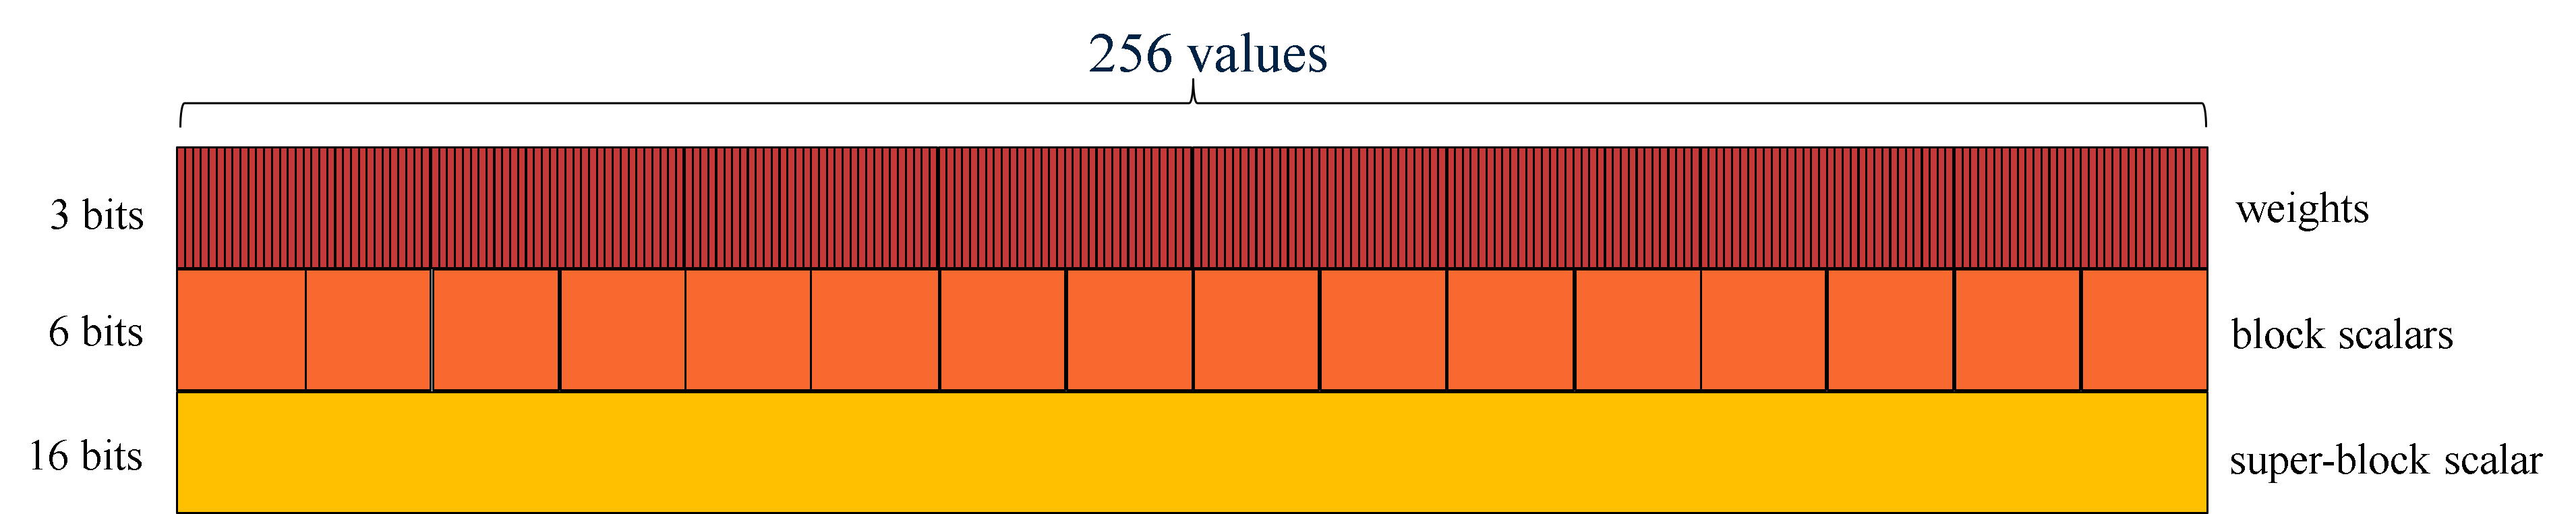
\includegraphics[width=0.9\columnwidth]{files/q3_k_formatv2.png} 
%         \caption{\label{fig:q3_k_format} Q3\_K super-block Data Format}
% \end{figure}

\subsection{Target Problem}

% We target the acceleration of MatMul operations, as they are the most computationally expensive in LLMs.
We target the acceleration of MatMul operations within our target LLM, as MatMul represents about $97\%$ of the computations.
Specifically, we accelerate the GGML's \qkernel kernel, which uses 3-bit weights and 8-bitinputs with BFP quantization.

% which is the core computation within BFP quantized MatMul; 

Both weights and inputs are stored in what is called "super-blocks" (SBs); these SBs are critical in maintaining LLM accuracy by adjusting mathematical scaling during computation.
With the \qkw format used for weights, each SB can represent 256 weights ($N_w$), where the SB is partitioned into 16 tiles ($N_{tiles}$) and each tile contains a scaling factor (6-bits) and 16 weights (3-bits). Additionally, each SB has one super-scaling factor (16-bits), which equates to $\sim$3.5 bits-per-weight.
% Equation~\ref{eq:sbw} can be used to calculate the number of bits for given super block of different quantisation schemes. 
With the \qki format, used for inputs, each SB contains 256 inputs (8-bits) and a single super-scaling factor \textit{SSF} (16-bits), which equates to 8$\sim$ bits-per-input.

% \begin{equation}\label{eq:sbw}
% \resizebox{.9\hsize}{!}{$
% SB_{bits} = N_d * (data_{bits}) + N_{tiles} * (scale_{bits}) + (SB\_scale_{bits})
% $}
% \end{equation}

% \begin{equation}
%     SBI_{size} = N_i * (8) + 16 = 2064~bits
% \end{equation}


%*********************************************************************************************

\subsection{Accelerator Design}

Our accelerator design, shown in Figure~\ref{fig:llm_acc}, contains an \emph{instruction decoder}, a \emph{data mapper}, a \emph{scheduler} and the \emph{Super-Block Vector Processor (SBVP)}:

\begin{itemize}
    \item The \emph{instruction decoder} loads and decodes instructions from the AXI-Stream and then communicates the instruction throughout the rest of the accelerator.
    
    \item The \emph{data mapper} parses the incoming data stream and maps the weight and input super-blocks into their respective weight and input buffers. 
    Our mapping scheme enables efficient data access, so that the \emph{SBVP} can compute without stalling the computation pipeline.
    
    \item The \emph{SBVP} efficiently computes the dot product between the SB of weights and inputs while scaling the computation according to the SB scaling factors.

    \item The \emph{scheduler} tiles the MatMul problem according to the dimension of the target layer. % and controls the \emph{SBVP}. 
    Additionally, it synchronizes and accumulates the output data produced by the SBVP and sends the results back to the main memory using the AXI-Stream.
\end{itemize}



% Our accelerator design, shown in Figure~\ref{fig:llm_acc}, contains an\emph{instruction decoder}, a \emph{data mapper}, a \emph{scheduler} and four \emph{vector processing units}.
% The \emph{instruction decoder} loads and decodes instructions from the AXI-Stream and then communicates the instruction throughout the rest of the accelerator.
% The \emph{data mapper} parses the incoming data stream and maps the weight and input super blocks into their respective weight and input buffers.
% Our mapping scheme enables efficient data access, so the \emph{vector processing units} can compute without stalling the computation pipeline.
% The \emph{vector processing units} efficiently compute the dot product between the SB of weights and inputs while scaling the computation according to the SB scaling factors.
% The \emph{scheduler} allocates SBs to each processing unit to process.
% Additionally, it synchronizes and accumulates the output data produced by the processing units and sends the results back to the main memory using the AXI-Stream.


\begin{figure}[!t]
 \centering
 % \includegraphics[width=0.95\columnwidth]{files/llm_acc2.pdf}
 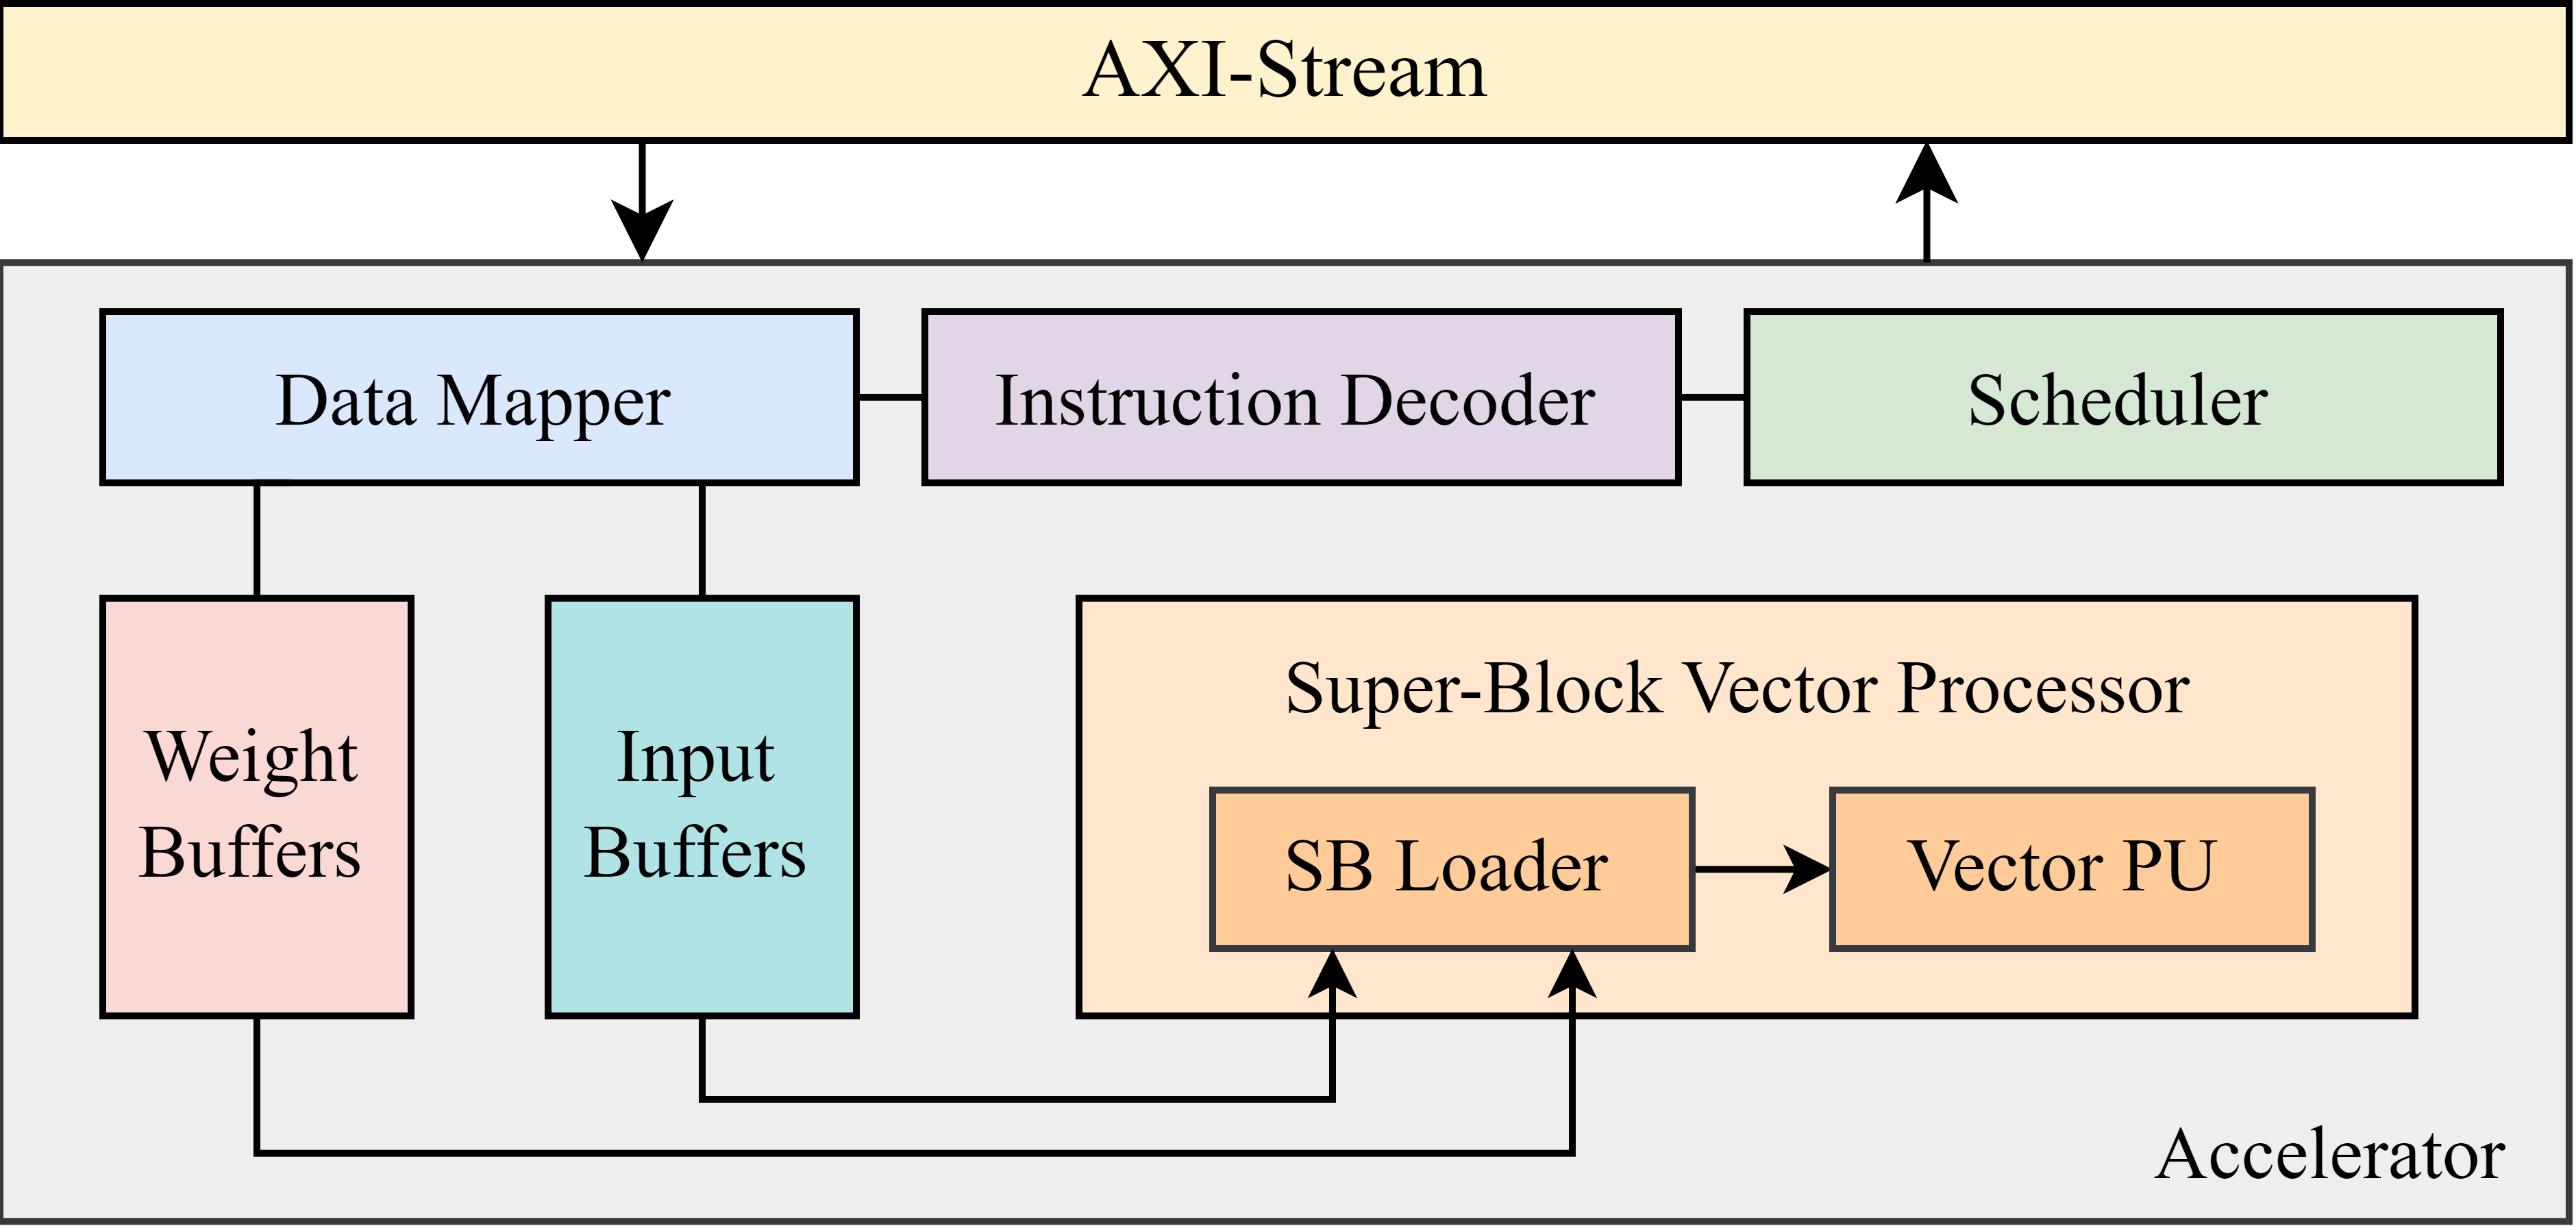
\includegraphics[width=0.95\columnwidth]{files/llm_acc4.png} 
  % \caption{\label{fig:llm_acc} Overview of our block floating point quantized accelerator design. It executes GGML's \qkernel kernel, where each vector processing unit is able to process up to 64 super-blocks at a time.}
    % \caption{\label{fig:llm_acc} Overview of our block floating point quantized accelerator design. It executes the GGML's \qkernel kernel, processing up to 64 super-blocks at a time.}
        \caption{\label{fig:llm_acc} Overview of our block floating point quantized accelerator design for GGML's \qkernel kernel.}
\end{figure}


%*********************************************************************************************


\subsection{Evaluation}
\label{subsubsec:exp_setup}

% \label{subsubsec:exp_setup}

We evaluate our accelerator design on the PYNQ-Z1 board~\cite{pynqz1}, which contains a Xilinx Z020 edge FPGA and a 650MHz dual-core Arm Cortex-A9 CPU.
We execute inference for the TinyLlama model~\cite{zhangTinyLlamaOpenSourceSmall2024}, that contains 1.1B parameters (460 MB), trained on the Guanaco dataset~\cite{joséphus_cheung_2023}.
This model contains various BFP quantization levels, but most layers are quantized to \qk.
Note that with~\LPP you can apply different levels of quantization to reduce model size as required.

% Note that with ~\LPP you can apply different levels of quantization to the same model to reduce model size as required.
% , \qk enabled reduction in model size in order to fit within our target board's memory.

For our experiments, we use the \LPP project's `main' program cross-compiled for our target CPU architecture, ARMv7a, with Neon vector instructions enabled alongside our accelerator driver.
We execute the TinyLlama model utilizing our FPGA-mapped accelerator to offload the \qkernel  layers, to obtain an initial speed of $1.7$ seconds per token ($\sim2$ seconds per word).
This provides a $11\times$ speedup over CPU-only inference, drastically improving the usability of LLMs on such a resource-constraint device. 
Therefore, with SECDA-LLM we could quickly implement, integrate and evaluate our new accelerator design.


% We execute the TinyLlama model (460 MB) utilizing our FPGA-mapped accelerator to obtain an initial speed of 20 seconds per token ($\sim$27 seconds per word).
% While this performance is just on par with the CPU for now, running TinyLlama on such a resource-constrained device was not possible a few months ago, and we expect to improve it in the future.
% With SECDA-LLM, we were able to implement, integrate and evaluate a new design quickly



% Note that while our design is an initial prototype, with SECDA-LLM, we were able to implement, integrate and evaluate a new design quickly.



% While this is slow for interactive use of the model, running TinyLlama on such a resource-constrained device was not possible few month prior.
% This is slow for interactive use of the model, but it demonstrates that with more optimizations running LLMs on this device would be feasible.


%*********************************************************************************************

% \subsection{Evaluation}\label{subsubsec:exp_setup}


% \subsubsection{Experimental Setup}
% % \label{subsubsec:exp_setup}

% We evaluate our accelerator design on the PYNQ-Z1 board~\cite{pynqz1}, which contains an edge FPGA and a 650MHz dual-core ARM Cortex-A9 CPU.
% We evaluate the TinyLlama model~\cite{zhangTinyLlamaOpenSourceSmall2024} with 1.1B parameters trained on the Guanaco dataset~\cite{joséphus_cheung_2023}.
% The model used contains various levels of float-based quantization, but the majority of layers are quantized to \qk weights.
% For evaluation, we make use of \LPP project's `main' program compiled for our target CPU architecture, ARMv7a with Neon vector instructions enabled.
% For our experiments, we have configured the \LPP's compilation flow to compile for ARMv7a with our accelerator driver enabled.


% %*********************************************************************************************

% \subsection{Results}

% Table~\todo{ref table with results} shows the key results of our evaluation.
% Comparing our accelerated inference to CPU only inference, we achieve a per token speedup of up to \uptopertokenX and and overall speedup of up to \uptooverallX.
% While our design is an initial prototype to demonstrate the capabilities of SECDA-LLM, we are able to achieve tangible performance improvement with minimal designer effort.
